\chapter{
	پیاده‌سازی سخت‌افزاری با
	\lr{Verilog}
}

\section{
	مقدمه
}

دنیای نرم‌افزار و سخت‌افزار رایانه در نگاه کلی می‌توانند بسیار شبیه به هم باشند، برنامه های نرم‌افزاری، مقادیری را به عنوان ورودی دریافت کرده، سپس طی روند مشخصی محاسباتی روی آنها انجام داده و در نهایت مقادیری را به عنوان خروجی به کاربر خود تحویل می دهند، قطعات سخت‌افزاری نیز دارای 
\lr{port}
هایی برای ارتباط با دنیای خارجی و دریافت ورودی‌ و تحویل خروجی‌های خود می‌باشند و از واحدهای مختلف پردازشی و عملیاتی مختلفی برای محاسبه ی خروجی‌های مناسب تشکیل شده اند. درعمل می‌توان سخت‌افزاری خاص برای اجرای بسیاری از روند های نرم‌افزاری طراحی و پیاده سازی کرد، ساخت سخت‌افزارِ خاصِِ مربوط به یک الگوریتم می تواند کاربرد‌های بسیاری داشته باشد، برای مثال قطعه‌ای که بتواند داده های ورودی را رمزنگاری کند می‌تواند به صورت گسترده برای ذخیره ی اطلاعات به صورت سریع استفاده شود، سخت‌افزار های اختصاصیِ الگوریتم ها سریع و بهینه اند و میتوانند به اجرای هرچه سریع تر روندهای پیچیده‌ای که به الگوریتم مورد نظر وابستگی فراوان دارند کمک کلانی کنند.

همانند بسیاری از الگوریتم‌های رایانه‌ای، الگوریتم تابعِ 
\lr{
	Skein Hashing
}
که در بخش قبل کلیتی از آنرا معرفی کردیم را می توان به صورت سخت افزاری پیاده‌سازی کرد، بدین صورت که قطعه‌ای طراحی و پیاده‌سازی کنیم که ورودی ای به اندازه ی دلخواه مارا دریافت و حاصل درهم‌سازی را به صورت خروجی ای به اندازه ی مورد نظر ما خروجی دهد. بر اساس نیاز و کاربرد ما از این قطعه، اندازه‌ی ورودی و خروجی را می توان ثابت و به مقدار دلخواه درنظر گرفت، سپس قطعه‌ای ثابت با پیاده سازیِ بهینه‌ای برای اندازه های مورد نظر طراحی کرد، یا این که قطعه‌ای  برای ورودی و خروجی های با اندازه های متغیر طراحی و پیاده سازی کرد. همان طور که در بخش قبل توضیح داده شد، تابع درهم‌سازی 
\lr{
	Skein Hashing
}
میتواند ورودی‌ای با اندازه ی دلخواه را دریافت کند و خروجی ای با اندازه‌ی دلخواه تحویل دهد، در این مقاله تمرکز ما روی پیاده سازی سخت‌افزاری حالتی از این تابع می باشد که اندازه ی بلاک های درونی تابع ( حالت درونی تابع ) 
\textbf{۵۱۲ بیت}
و حاصل درهم‌سازی نیز به صورت خروجی ای به اندازه ی 
\textbf{۵۱۲ بیت}
می باشد، این تابع در اصطلاح 
\lr{
	\textit{Skein 512-512}
}
نامیده می‌شود.

مراحل طراحی و پیاده‌سازی سخت‌افزاری یک قطعه معمولا به آن صورت است که برای اطمینان از کارکرد صحیح پیاده‌سازی، موازی با طراحی سخت‌افزاری قطعه، پیاده سازی دیگری از الگوریتم به نام مدل طلایی انجام می‌شود و پس از پایان طراحی‌ها، کارکرد قطعه با مدل طلایی مقایسه می شود تا قطعه‌ی نهایی مشکلی نداشته باشد. در بخش 
\hyperref[chapter:GoldenModel]{\textbf{مدل طلایی}}
به تفصیل درباره‌ی مدل طلایی استفاده شده در این پروژه توضیح داده شده است. در این بخش به پیاده‌سخت‌افزاری این الگوریتم به کمک زبانِ توصیف سخت‌افزارِ 
\lr{Verilog}
می پردازیم.

\pagebreak
\section{
	پیاده‌سازی
}
همان طور که توضیح داده شد، الگوریتم 
\lr{Skein}
از سه بخش اصلی تشکیل می‌شود:
\begin{itemize}
	\item 
	\lr{\textit{\textbf{Threefish}}} 
	یا بلاک های رمزنگاری قابل تنظیم،
	\item
	\lr{
		\textit{
			\textbf{Unique Block Iteration (UBI)}
		}
	}
که یک حالت زنجیره ای است که از
\lr{Threefish}
به صورتی استفاده می کند که ورودیِ ‌به اندازه‌ی دلخواه به خروجی‌ای به اندازه‌ای مشخص تبدیل شود.
\item
\textbf{\lr{\textit{\textbf{Optional Argument System}}} } 
که به الگوریتم توانایی پشتیبانی از بسیاری ویژگی های دلخواه را، بدون افزودن باری اضافه به پیاده سازی الگوریتم می‌دهد.

\end{itemize}

طراحی ای که ما در این پروژه به بررسی‌اش می‌پردازیم، یک طراحی بسیار ساده شده از الگوریتمِ
\lr{Skein 512-512}
می باشد. در این طراحی اندازه ی ورودیِ و خروجی اش ثابت و ۵۱۲ بیت می باشند، و اندازه ی حالت درونی تابع درهم‌سازی نیز دقیقا برابر اندازه‌ی ورودی و خروجی‌هاست، بنابراین در این طراحی اثری از پیاده‌سازی یک 
\lr{UBI}
 پیچیده نیست. علاوه‌ بر این، این پیاده‌سازی، پیاده‌سازی خام خود الگوریتمِ
 \lr{Skein 512-512}
 بوده و هیچ ویژگی اضافی ای را پشتیبانی نمی‌کند، بنابراین اثری از پیاده‌سازی 
\lr{Optional Argument System}
نیز در آن نیست. بنابراین طراحی، صرفا شامل بلاک های رمزنگاری قابل تنظیم بوده، داده‌ی ورودی به صورت مستقیم با این بلاک ها تزریق شده و خروجی الگوریتم نیز به صورت تقریبا مستقیم از آخرین بلاک دریافت می‌شود.

\subsection{
	بررسی درستی طراحی ارائه شده
}
طراحی‌ای که دراختیار ما قرار گرفته بود 
(
\href{https://github.com/VahidZee/SkeinHashingHDL/blob/master/SourceCode/Verilog/skein.v}{این فایل} 
)
، شامل مشکلات منطقی فراوان بود، مشکلات موجود در هر خط از کد 
\lr{verilog}
به صورت یک 
\lr{comment}
در قالب 
$$todo: <Valid Code>$$
مشخص شده اند، علاوه بر این طراحی تصحیح شده 
(
\href{https://github.com/VahidZee/SkeinHashingHDL/blob/master/SourceCode/Verilog/corrected.v}{این فایل} 
)
نیز در کنار مقاله پیوست شده است، تمامی مستند سازی های این مقاله، براساس پیاده سازی تصحیح شده ی کدهای اولیه می‌باشد.
\subsection{
	ساختار طراحی
}
ساختار کلی طراحی شده برای این الگوریتم به سه بخش که در تصویر زیر قابل مشاهده اند قابل تفکیک است، ماژول اصلی طراحی که 
\lr{skein512}
نام گذاری شده است، این سه وظیفه را بر‌عهده دارد.
\vspace{-0.2cm}
\begin{figure}[H]
	\centering
	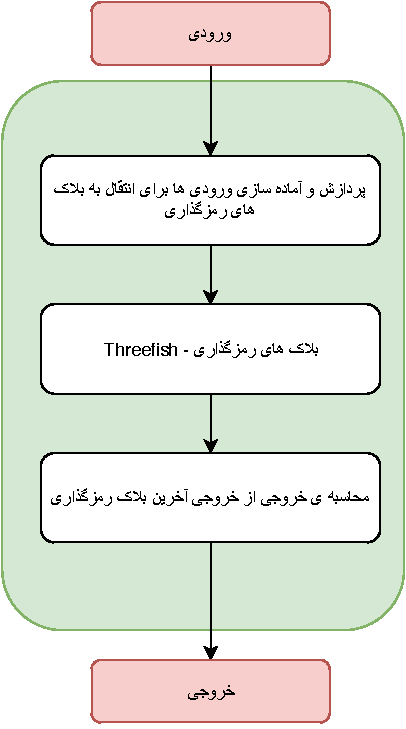
\includegraphics[width=3.5cm]{Images/VerilogDocumentation/skein_functionality.pdf}	
	\caption{ساختار کلی پیاده‌سازی سخت‌افزاری}
\end{figure}
دو بخش پردازش ورودی و خروجی‌ها به صورت کامل در ماژول 
\lr{skein512}
صورت می گیرند و به تفصیل درباره ی آنها توضیح داده خواهد شد، بخش بلاک های رمزگذاری از ماژول های 
\lr{skein\_round} 
و 
\lr{skein\_round\_1} 
تا 
\lr{skein\_round\_4} 
تشکیل شده و قرارگیری زنجیره‌ای آنها و محاسبه ی اولیه‌ی مقادیر کلید‌های رمزنگاری در ماژول 
\lr{skein512}
صورت گرفته است.

\subsection{
	پیاده سازی بلاک‌های رمزگذاری
}
همان‌طور که در معرفی الگوریتمِ
\lr{Skein Hashing}
در بخش اول توضیح داده شد، این الگوریتم برای تولید مقدار درهم‌سازی از بلاک های رمزگذاری که به صورت زنجیره ای یکی پس از دیگری قرار گرفته اند، استفاده می کند و این بلاک‌ها بخش عمده‌ای از طراحی سخت‌افزاری را دربر می‌گیرند. 

شمای کلی حرکت داده داخل بلاک های رمزنگاری در این الگوریتم به شکل زیر می باشد:
\begin{figure}[H]
	\centering
	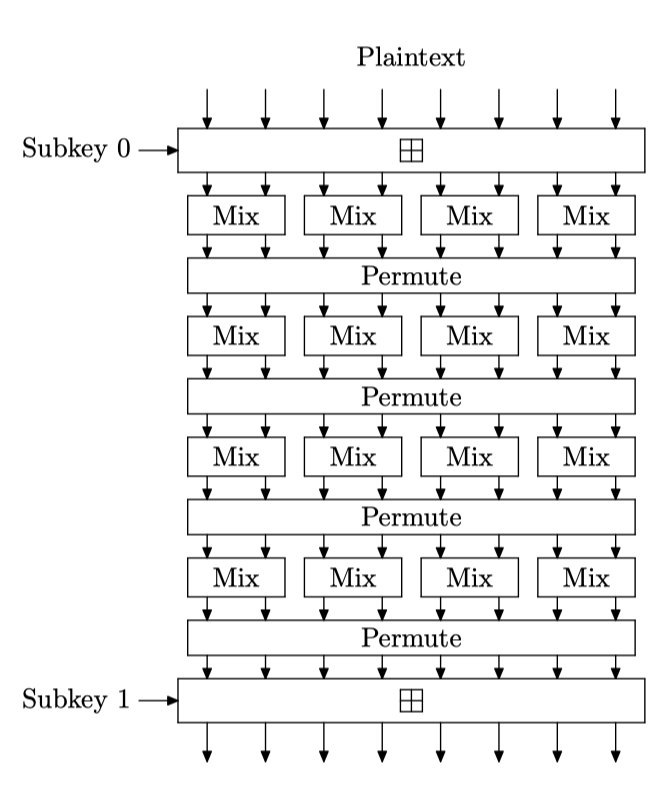
\includegraphics[width=7cm]{Images/VerilogDocumentation/cipherblock_dataflow.png}	
	\caption{شمایی از حرکت داده در بلاک های رمزنگاری}
\end{figure}
داده‌ی ورودی که به ۸ بخشِ ۶۴ بیتی تقسیم می‌شود، به بلاک‌های رمزنگاری تزریق شده و پس از ۴ مرحله ی متوالی از درهم‌سازی 
(
\lr{Mix}
)
و
 جابه‌جایی 
 (
 \lr{Permutation}
 )
 - که به هر‌ یک از آنها یک
 \lr{\textit{round}}
 می‌گوییم -  
 با مقادیری به نام 
\lr{\textit{Subkey}}
که از کلید‌های رمزنگاری - که آنها نیز از ۸ بلاک ۶۴ بیتی تشکیل شده اند - به دست می‌آیند، جمع می‌شوند.

محاسبات دقیق
\lr{Subkey}
ها و توابعِ غیرخطی 
درهم‌سازی 
(
\lr{Mix}
)
و
جابه‌جاییِ 
(
\lr{Permutation}
)
 هر
\lr{round}
به تفصیل در بخش اول مقاله، توضیح داده شده است. آن چیزی که در‌این میان حائز اهمیت است، استفاده‌ای هوشمندانه از نظم تکراری این توابع محاسباتی در پیاده‌سازی سخت‌افزاری مورد بررسی ما در این مقاله است.
\pagebreak

\subsubsection{
	پیاده سازی توابع جابه‌جایی 
	(
	\lr{Permutation}
	)
	هر
	\lr{round}
}
 تابع غیرخطیِ جابه‌جایی
(
\lr{Permutation}
)
یک عملیات ثابت را روی مقادیر خروجی از توابع درهم‌سازی
(
\lr{Mix}
)
انجام می‌دهد، این تابع در ماژول‌های 
\lr{skein\_round\_1} 
تا 
\lr{skein\_round\_4} 
به صورت توصیف رفتاری با کمک یک 
\lr{always block}
حساس به لبه‌ی بالا‌رونده‌ی ساعت پیاده سازی شده است.
مقادیر خروجی توابع درهم‌سازی (
\lr{Mix}
)
مربوط به هر ماژول - که جلوتر پیاده‌سازی آنها را بررسی خواهیم کرد -، به هنگام لبه‌ی بالارونده ی ساعت، جابه‌جا شده و به خروجی ماژول انتقال داده می‌شوند. 


توصیف ارائه شده از جابه‌جایی 
(
\lr{Permutation}
)
در این 
\lr{always block}
ها در واقع معرف مجموعه ای از ۵۱۲ 
\lr{D-FlipFlop}
 حساس به لبه‌ی بالا‌رونده ی ساعت می باشد.
 
 \subsubsection{
 پیاده سازی توابع درهم‌سازی 
 (
 \lr{Mix}
 )
 هر
 \lr{round}
}
برخلاف توابع جابه‌جایی (
\lr{Permutation}
) که یک عملیات ثابت را در هر 
\lr{round}
اجرا می‌کنند، این توابع غیر‌خطی، بر اساس این که در کدام
\lr{round}
قرار دارند،‌ محاسبات خاص خود را خواهند داشت، همان طور که در بخش قبل توضیح داده شد، هر درهم‌سازی (
\lr{Mix}
) شامل، یک جمع، یک گردش به چپ و یک
\lr{xor}
می باشد. جمع و \lr{xor} ها در همه‌ی \lr{round} ها یکسان‌ اند و به صورت یکتا پیاده می‌شوند.

 چیزی که در هر
 \lr{round}
  متفاوت خواهد بود، تعداد گردش ها به چپ می‌باشد،
با توجه به مقادیر ارائه شده و فورمول‌های توضیح داده شده در بخش قبل، این مقادیر هر ۸ 
\lr{round}
 تکرار می شوند، مسئله ی دیگر آن است که قرار است هر ۴ 
 \lr{round}
 ،
\lr{subkey}
   های مربوطه به مقادیر موجود در بلاک‌های رمزگذاری افزوده شوند، برای همین در پیاده‌سازی مورد بررسی ما هر ۴ 
\lr{round}
   در یک ماژول به نام
    \lr{skein\_round}
    در نظر گرفته شده است و پیاده سازی خود 
     \lr{round} 
     ها در ماژول های  
     \lr{skein\_round\_1} 
     تا 
     \lr{skein\_round\_4} 
     تعریف شده اند.
     این بدین معنا است که برای دوره ی تناوب ۸ تایی توابع درهم‌سازی (
     \lr{Mix}
     ) هر 
     \lr{round}
     ، صرفا دانستن این که در ۴  \lr{round} شماره ی فرد یا زوج قرار داریم برای ماژول های 
     \lr{skein\_round\_1} 
     تا 
     \lr{skein\_round\_4} 
     کافی می باشد. برای همین این ماژول‌ها یک ورودی تک بیتی به نام
     \lr{even}
     دریافت می کنند و بر اساس آن تعداد گردش به چپ‌های مناسب را بر می گزینند.
     
     پیاده‌‌سازی خود توابع درهم‌سازیِ (
     \lr{Mix}
     ) هر 
     \lr{round}
   ، در دو بخش در ماژول های 
    \lr{skein\_round\_1} 
    تا 
    \lr{skein\_round\_4} 
تعریف شده است.
در بخش اول عملیات‌های جمع و گردش به چپ‌ها به توصیفی ساختاری و به کمک یک سری 
\lr{continuous assignment} 
در این ماژول‌ها مشخص شده‌ اند، لازم به ذکر است که در 
\lr{verilog}
عملگر گردش به چپ وجود ندارد، برای همین برای پیاده سازی گردش به چپِ یک \lr{vector}، از ترکیب \lr{part selection} و \lr{concatenation} استفاده شده است.
 در بخش دوم عملیات‌های
\lr{xor}
هم‌زمان با عملیات‌های جابه‌جایی (
\lr{Permutation}
)
در 
\lr{always block}
مربوط به آنها در این ماژول‌ها معرفی شده است.

توصیف ارائه شده از توابع درهم‌سازی (
\lr{Mix}
) 
در عمل معرف مجموعه ای از مدار‌های ترکیبی (
\lr{combinational}
) می باشد و منجر به تولید گیت‌های منطقی مستقل از سیگنال ساعت خواهد شد.

\subsubsection{
	پیاده سازی 
	\lr{round}
	ها
}
همان طور که بار ها گفته شد \lr{round} شامل درهم‌سازی 
(
\lr{Mix}
)
و
جابه‌جاییِ 
(
\lr{Permutation}
)
روی ورودی‌هایش می‌باشد که به تفصیل به پیاده سازی این دو تابع غیرخطی در طراحی مورد بررسی‌مان پرداختیم، تنها مسئله ی مجهول شیوه‌ی اتصال این دو بخش در ماژول های 
 \lr{skein\_round\_1} 
تا 
\lr{skein\_round\_4} 
و تشکیل واحد های محاسباتی \lr{round} های الگوریتم می‌باشد که بلاک دیاگرام های تهیه شده در تصاویر دو صفحه‌ی بعدی به تفصیل این مسئله و هم‌چنین شمای کلی حرکت داده داخل این ماژول‌ها را توضیح می دهند:
\begin{figure}[H]
	\centering
	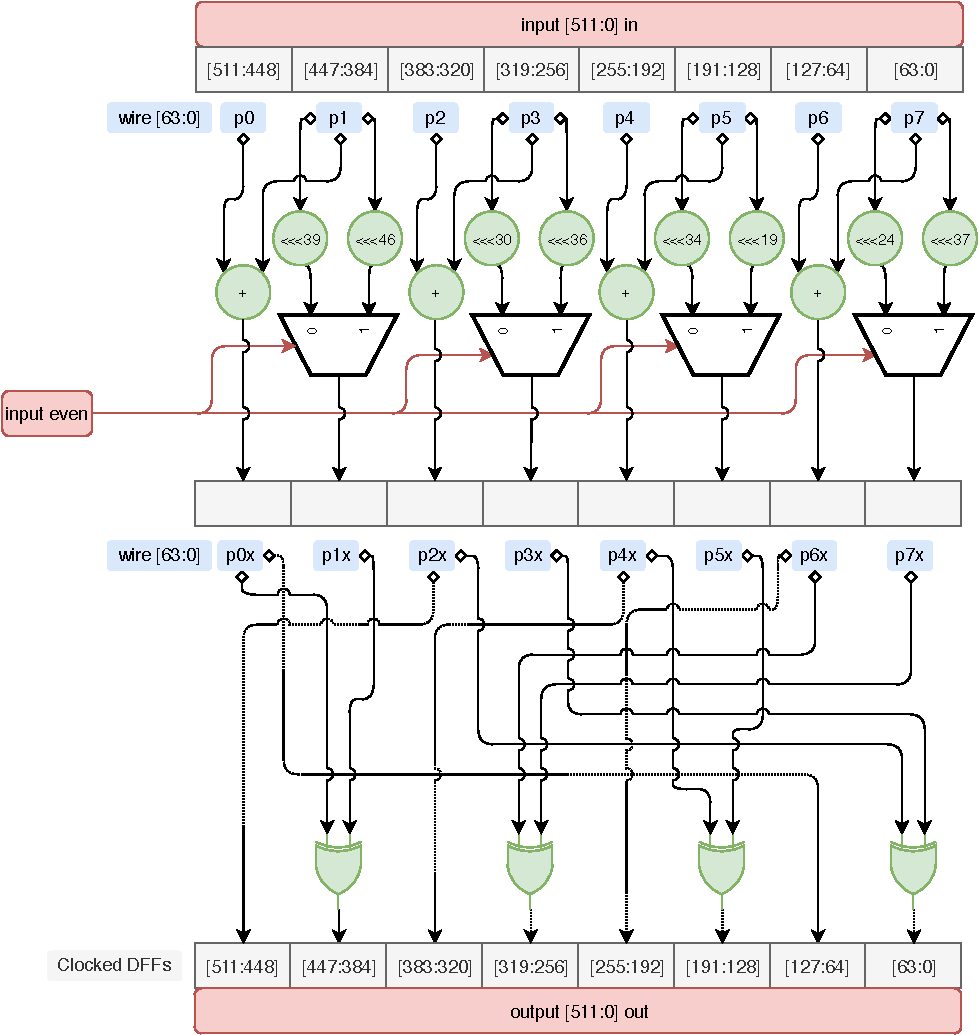
\includegraphics[width=10.5cm]{Images/VerilogDocumentation/diagrams_round1.pdf}	
	\caption{
	بلاک دیاگرام شماتیک و نحوه‌ی جریان داده در ماژول 
	\lr{skein\_round\_1}
}
\end{figure}
\begin{figure}[H]
	\centering
	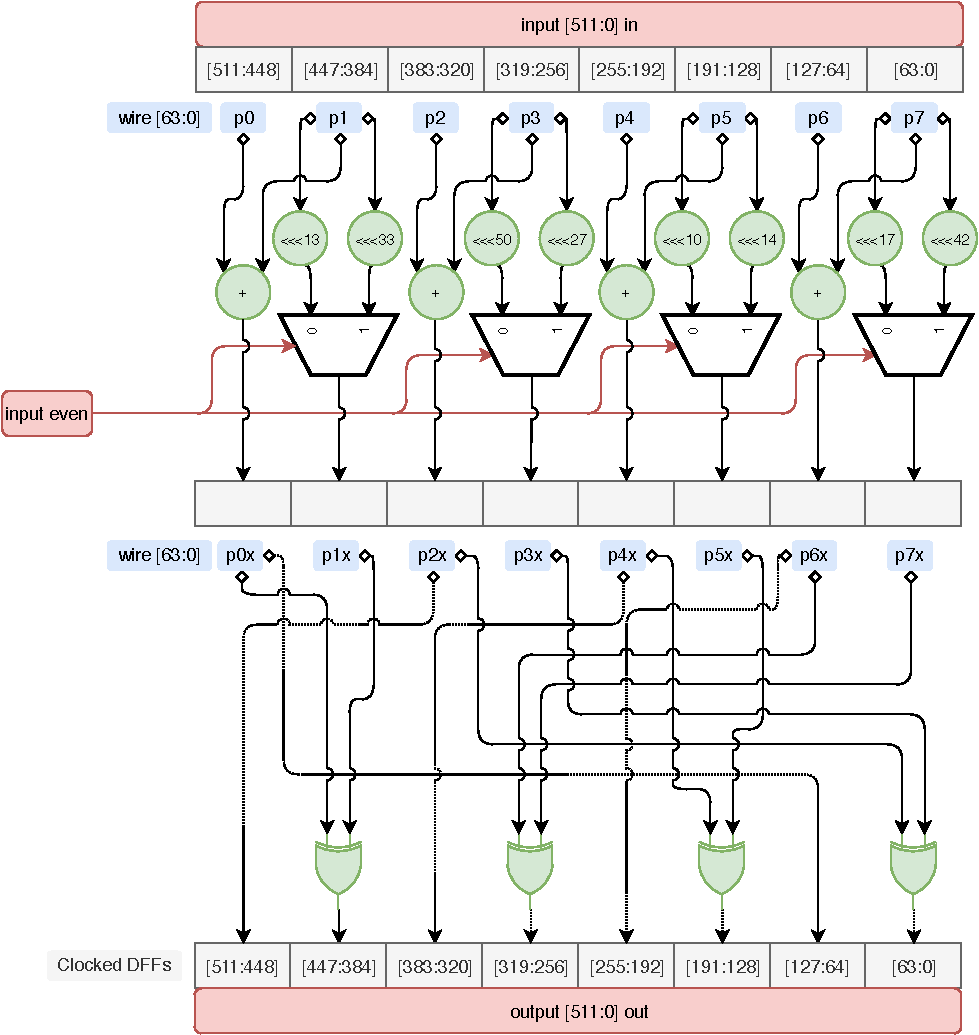
\includegraphics[width=10.5cm]{Images/VerilogDocumentation/diagrams_round2.pdf}	
	\caption{
		بلاک دیاگرام شماتیک و نحوه‌ی جریان داده در ماژول 
		\lr{skein\_round\_2}
	}
\end{figure}
\begin{figure}[H]
	\centering
	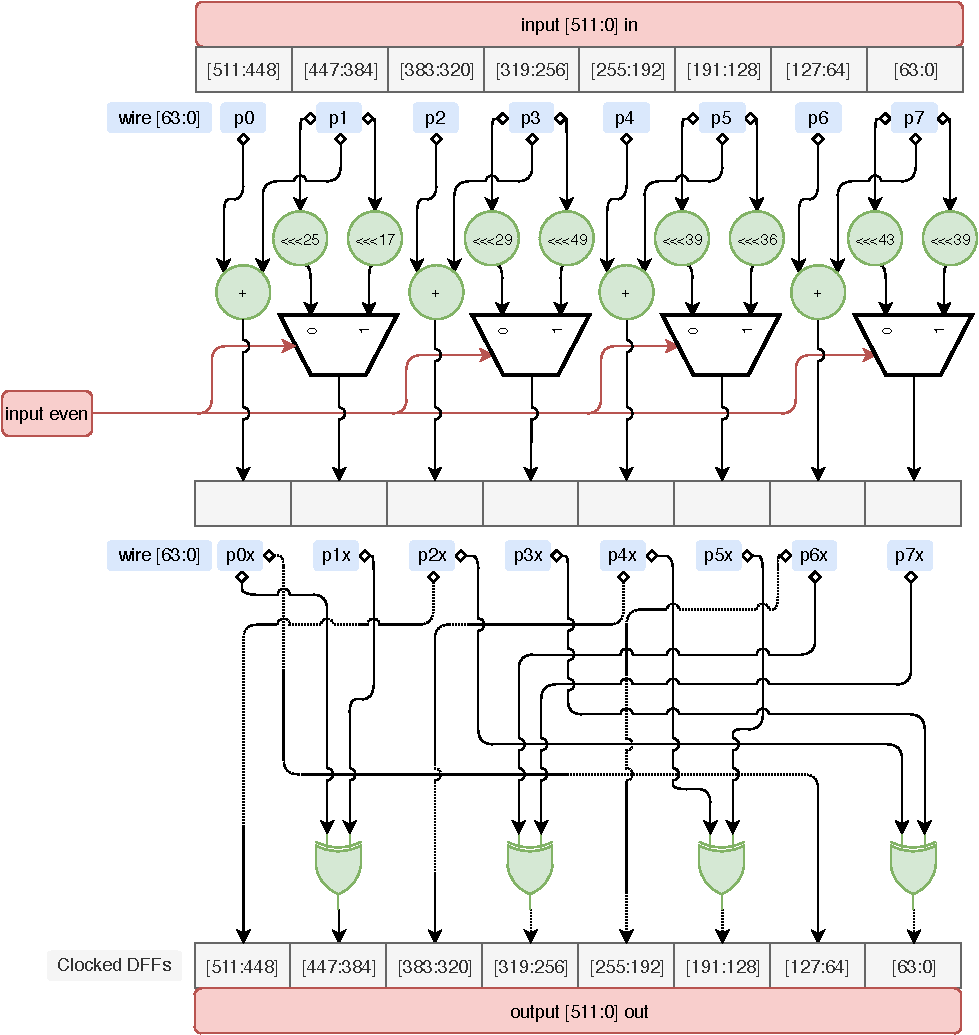
\includegraphics[width=10.5cm]{Images/VerilogDocumentation/diagrams_round3.pdf}	
	\caption{
		بلاک دیاگرام شماتیک و نحوه‌ی جریان داده در ماژول 
		\lr{skein\_round\_3}
	}
\end{figure}
\begin{figure}[H]
	\centering
	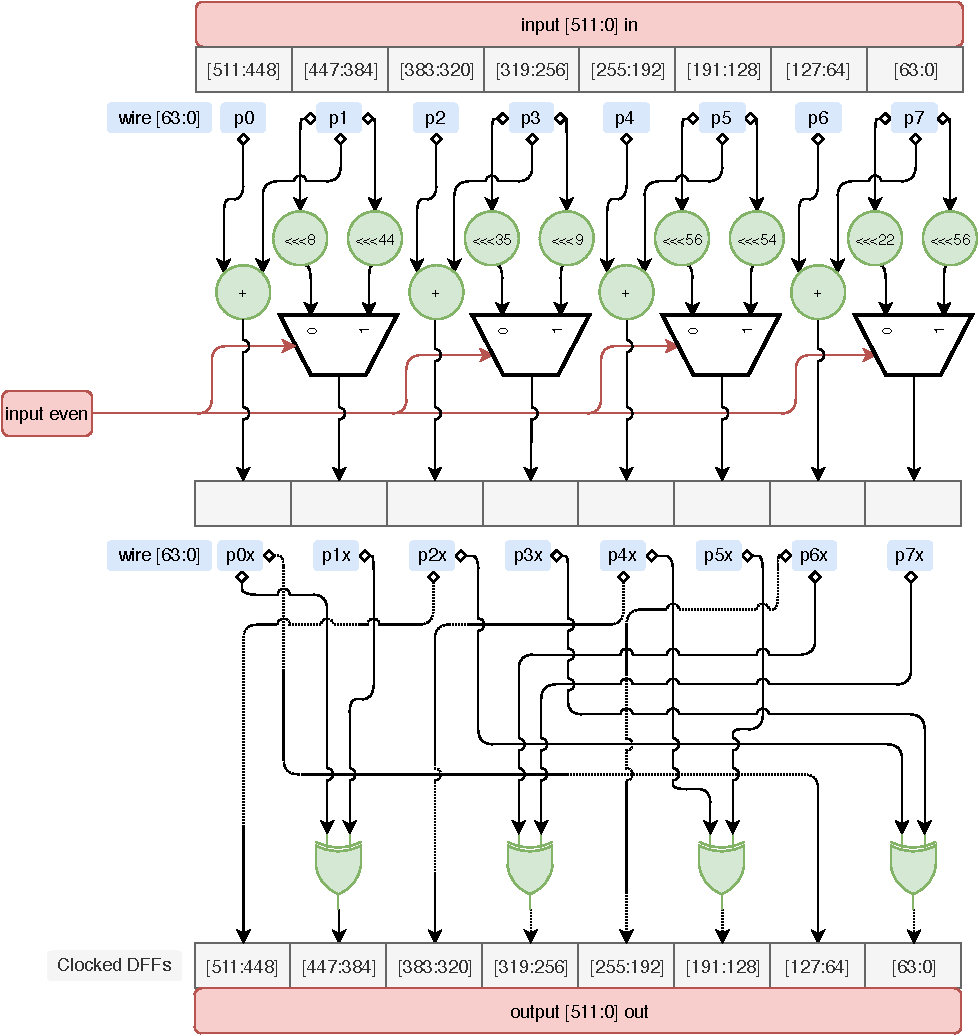
\includegraphics[width=10.5cm]{Images/VerilogDocumentation/diagrams_round4.pdf}	
	\caption{
		بلاک دیاگرام شماتیک و نحوه‌ی جریان داده در ماژول 
		\lr{skein\_round\_4}
	}
\end{figure}

\subsubsection{
	محاسبه و افزودن 
	\lr{Subkey}
	ها
}
همان‌طور که اشاره شد، قبل از هر ۴
\lr{round}
مقادیری به نام 
\lr{Subkey}
به مقادیر محاسبه شده در بلاک‌های رمزگذاری افزوده می‌شود، طبق توضیحات بخش اول، مقادیر 
%todo reference
\lr{Subkey}
‌ها باتوجه به شماره‌ی
\lr{round}
تنظیم می‌شوند، اگر به فورمول محاسبه‌ی 
\lr{Subkey}
ها توجه کنید
%todo formula refrence
متوجه دو تناوب خواهید شد، یکی برای خود مقادیر 
\lr{Subkey}
ها که پس از هر‌بار محاسبه‌، انگار که یک خانه جا‌به‌جا شوند، دیگر آنکه پس از هر‌ ۳ 
\lr{round}
جای مقادیر تنظیم
\lr{tweak} 
(
$t_0$ , $t_1$ , $t_2$
)
یک دور کامل می‌چرخند.

ماژول 
\lr{skein\_round}
 شامل ۴ 
 \lr{round}
 متوالی از بلاک‌های رمزگذاری و واحد افزودن مقادیر 
 \lr{Subkey}
 ها به مقادیر محاسبه شده در بلاک‌های رمزگذاری قبلی و هم‌چنین پیاده‌سازیِ یکی از این دو دوره‌ی تناوب می‌باشد. 
 به صورت خلاصه تصویر زیر معرف شمای کلی و نحوه‌ی جریان داده ها در هر نمونه از ماژول‌های
 \lr{skein\_round}
 می‌باشد:
 \begin{figure}[H]
 	\centering
 	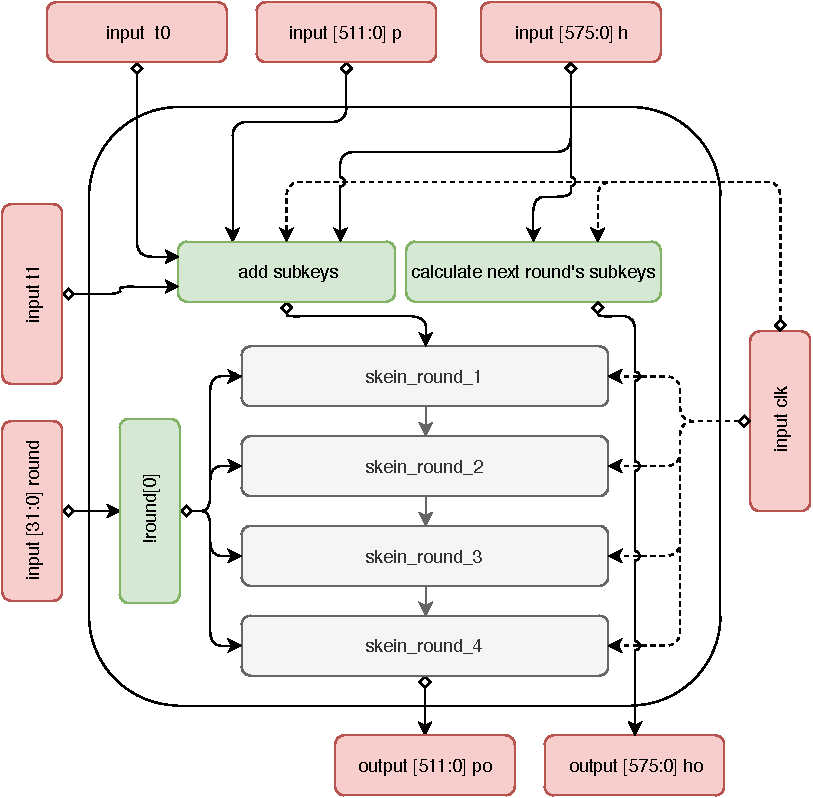
\includegraphics[width=10cm]{Images/VerilogDocumentation/skeinround_dataflow.pdf}	
 	\caption{شمایی از نحوه‌ی حرکت داده و ساختار هر نمونه از ماژول
 	\lr{skein\_round}
 }
 \end{figure}
ورودی 
\lr{input [575:0] h}
به ترتیب از سمت با‌ارزش‌ترین بیت، شامل
\lr{Subkey}
های مربوط به این 
 \lr{round}
 یعنی:
 $$Subkey_{round,\ 0}, Subkey_{round,\ 1}, Subkey_{round,\ 2}, ..., Subkey_{round,\ 8}$$
و ورودی های 
\lr{input t0}
و
\lr{input t1}
به ترتیب حاوی مقادیر تنظیم (
\lr{tweak}
)
مربوط به این 
 \lr{round}
، یعنی:
$$t0 = t_{ round \ mod \ 3 } $$
$$t1 = t_{ (round + 1 ) \ mod \ 3}$$
 می باشد. بنابراین این ورودی ها بدون هیچ پیش‌پردازشی آماده‌ی تزریق به بخش افزایش به مقادیر رمزگذاری شده در 
 \lr{round}
 های قبلی می‌باشند.  بخش افزاینده‌ی مقادیر 
\lr{Subkey}
ها به مقدار رمزگذاری شده از بلاک‌‌(ها)ی قبلی ، در این ماژول،  با توجه به فورمول محاسباتی توضیح داده شده در بخش قبل، محاسبات مربوط به این 
 \lr{round}
 را از روی ورودی های خود انجام می‌دهد. 
پیاده‌سازی این بخش در کد با توصیفی رفتاری به کمک یک 
\lr{always block}
حساس به لبه‌ی بالارونده‌ی ساعت مشخص شده است. این توضیحات بخش اول توصیفات موجود در این 
\lr{always block}
بوده و در عمل معرف ترکیبی از یک مداری ترکیبی (‌برای محاسبات جمع 
\lr{Subkey} 
ها‌و مقادیر رمزگذاری شده‌ي 
\lr{p}
) و مداری ترتیبی (برای انتقال حاصل عملیات‌های جمع به ورودی 
\lr{skein\_round\_1}
) می‌باشد.

بخش دیگری که در این ماژول پیاده‌سازی شده است، محاسبه‌ی 
\lr{Subkey}
های مربوط به
 \lr{round}
 بعدی براساس 
 \lr{Subkey}
 های این 
  \lr{round}
  می‌باشد.
  اگر به فورمول های محاسبه‌ی
  \lr{Subkey}
  ها توجه کنید، واضح است که پس از هر 
   \lr{round}
   انگار  \lr{Subkey}
   ها یک گردش به چپ دارند. دقیقا همین ایده در این ماژول به کمک توصیفی رفتاری در بخش دوم کد های 
   \lr{always block}
   حساس به لبه‌ی بالارونده‌ی ساعت، پیاده شده‌است. این توصیف در واقع معرف یک مدار ترکیبی برای محاسبه ی حاصل 
   \lr{xor}
   $Subkey_{round,\ 0}$
   تا
$Subkey_{round,\ 7}$
و یک مدار ترتیبی برای انتقال مقادیر یک بلاک چرخش به چپ و حاصل 
\lr{xor}
\lr{Subkey}
ها به خروجی می باشد.

پیاده‌سازی و مقدار‌دهی تناوبی مقادیر تنظیم (
\lr{tweak}
)
به هنگام نمونه‌گیری ماژول‌های 
\lr{skein\_round}
در ماژول اصلی یعنی
\lr{skein512}
انجام شده است.

\subsubsection{
	اتصال 
	\lr{round}
	ها به یکدیگر و پیاده‌سازی بلاک های رمزگذاری به صورت زنجیره‌ای
}
در پیاده‌سازی الگوریتم
\lr{Skein 512-512}
برای محاسبه‌ی مقدار درهم‌سازی نهایی باید ۷۲ 
\lr{round}
بلاک‌های رمزگذاری پشت‌سر‌هم به صورت یک زنجیره تکرار شوند، پیاده‌سازی این مسئله در ماژول 
\lr{skein512}
که بالاترین ماژول طراحی مورد بررسی ما است، صورت می‌گیرد.

این‌کار به صورت ترکیبی از توصیف های ساختاری و رفتاری در این ماژول انجام شده است،
کنارهم قرارگرفتن بلاک‌های رمزگذاری به توصیفی ساختاری با نمونه گیری از ۱۸ ماژول 
\lr{skein\_round}
انجام شده است. همان‌طور که در بخش قبل توضیح داده شد، محاسبات مربوط به 
\lr{Subkey}
ها، دارای دو تناوب هستند، یکی از این تناوب ها در محاسبات داخل خود ماژول های 
\lr{skein\_round}
صورت می‌گیرد که به تفصیل درباره‌ی آن توضیح داده شد. تناوب دومِ محاسباتی مربوط به انتخاب تنظیم (
\lr{tweak}
)مناسب بین سه تنظیم
$t_0,\ t_1,\ t_2$ 
می‌باشد. این تناوب هنگام نمونه‌گیری ماژول های
\lr{skein\_round}
در ماژول
\lr{skein512}
صورت گرفته است و چرخش ۳ تا ۳ تای مقادیر تنظیم اختصاص داده شده به 
\lr{port}
های ماژول های 
\lr{skein\_round}
، به وضوح قابل مشاهده است.

در بخش دیگر، اتصالات این ماژول هایی که نمونه‌گیری می‌شوند توصیف شده اند. در یک 
   \lr{always block}
   حساس به لبه‌ی بالا‌رونده‌ی ساعت، خروجی هر‌یک از ماژول های
   \lr{skein\_round}
   به ورودی ماژول
     \lr{skein\_round}
     بعدی خود متصل شده است. این پیاده سازی در عمل مداری کاملا ترتیبی است و موجب قرار‌گیری یک سری 
     \lr{D-FlipFlop}
     حساس به لبه‌ی بالا‌رونده‌ی ساعت بینِ ماژول های  
      \lr{skein\_round}
      می‌شود که سرِ هر سیگنال بالا‌رونده‌ی ساعت، خروجی هر 
           \lr{skein\_round}
           را
           به ورودی 
                \lr{skein\_round}
                بعدی منتقل می کند.
                
\subsection{
پیاده‌سازی بخش پردازش ورودی اولیه و خروجی نهایی
}
همان‌طور که در توضیحات اخیر اشاره شد، ماژول اصلی طراحی،
\lr{skein512}
علاوه بر دربرداشتن کل بلاک‌های رمزگذاری، ورودی ها را برای تزریق به این بلاک ها پیش‌پردازش کرده و خروجی مناسب را از خروجی آخرین بلاک رمزگذاری تولید می‌کند. پیاده‌سازی این بخش بسیار واضح و سرراست است، از روی مقادیر 
\lr{nonce}
و 
\lr{data}
مقدار ورودی اولیه به بلاک های رمزگذاری محاسبه می شود که پیاده سازی این بخش عمدتا به صورت توصیفی رفتاری از مدار ترکیبی در یک 
\lr{always block}
صورت گرفته است. این 
\lr{always block}
مدار 
\lr{skein512}
دارای دو حالت کلی است که با یک فلیپ فلاپ به نام
\lr{phase}
مشخص شده است، مقدار کنونی
 \lr{phase}
 \lr{phase\_q}
 و مقدار بعدی آن 
 \lr{phase\_d}
 به کمک این معرفه‌ی حالت، مدار بین هر پالس ساعت دو عملکرد متفاوت تزریق کلید‌ها و تنظیمات و داده ها را به بلاک های رمزگذاری انجام می‌دهد.
 
 علاوه بر محاسبه ی ورودی و کلید‌ها و تنظیمات مناسب - از روی ورودی های ماژول - برای بلاک های رمزگذاری قابل تنظیم، ماژول 
  \lr{skein512}
  از این بلاک‌‌های رمزگذاری خروجی ای به عنوان مقدار درهم‌سازی شده از ورودی ها به ما خواهد داد، پیاده‌سازی محاسبات مربوط به استخراج خروجی نهایی همانند مجاسبات مربوط به پیش‌پردازش ورودی ها سر‌راست و ساده است، پس از محاسبه و افزودن یک سری دیگر از 
  \lr{Subkey}
  ها (کلید‌های طبقه‌ی شماره‌ی ۱۸ یا درواقع ۱۹ ام) به مقادیر خروجی از بلاک‌های رمزگذاری که توصیف آنها در بخش دوم
 \lr{always block}
  معرف مدار ترکیبی ماژول آمده است،
 به کمک توصیف ساختاری و با استفاده از
  \lr{part selection}
  و 
  \lr{continuous assignment}
  بایت‌های مقدار محاسبه‌شده پس از افزودن سری ۱۹ام کلید‌ها، جایگشت کاملا تازه ای به خود گرفته و به عنوان خروجی الگوریتم مشخص می شوند.
  
  بنابراین بخش محاسبه‌ی خروجی نهایی ماژول، شامل یک بخش محاسبه و افزاینده ی کلید‌های سری ۱۹ام به مقادیر محاسبه‌شده در بلاک‌های رمزگذاری و بخشی برای جابه‌جایی مقدار محاسبه شده می‌باشد، این پیاده‌سازی ها در عمل کاملا معرف مدار‌هایی ترکیبی می‌باشد.
  
  \subsection{ 
جمع‌بندی
  }
بنابر توضیحات ارائه شده در این بخش، ساختار کلی و دقیق طراحی سخت‌افزاری الگوریتم مشخص شد. از دید ساختار درختی، این طراحی  از ۶ ماژول تشکیل تشکیل می‌شود که ارتباط کلی آنها در تصویر زیر قابل مشاهده‌است:

 
 \begin{figure}[H]
 	\centering
 	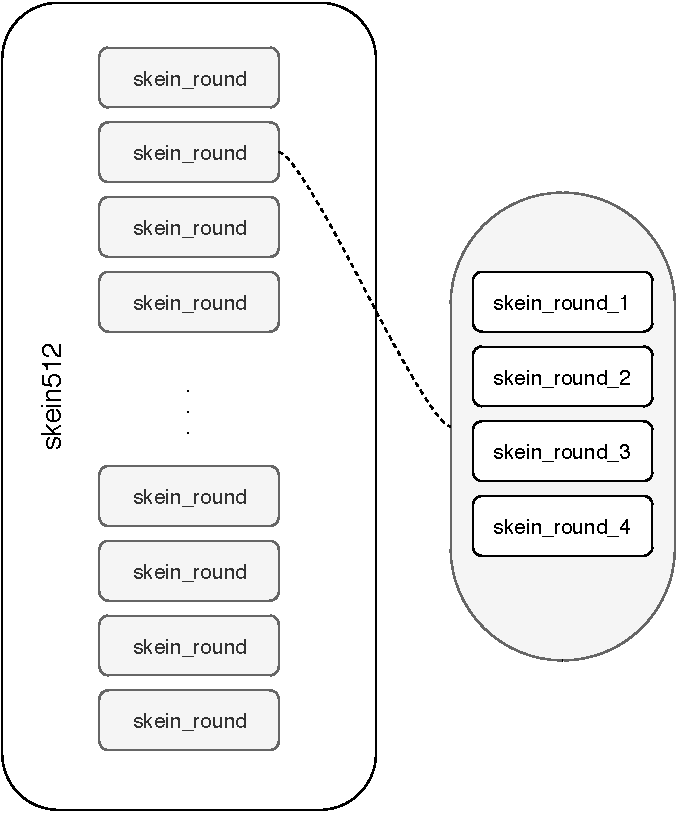
\includegraphics[width=10cm]{Images/VerilogDocumentation/modules_hierarchy.pdf}	
 	\caption{
 		نموداری از ساختار درختی و روابط ماژول ها با یکدیگر در طراحی
 	}
 \end{figure}
\section{
شبیه‌سازی
}
در مراحل طراحی قطعات سخت‌افزاری، پیش از تولید نهایی قطعات، به کمک نرم‌افزار‌های شبیه‌ساز، طراحی انجام شده شبیه‌سازی می شود. برای انجام شبیه‌سازی لازم است نحوه ی ورودی و خروجی گرفتن از طراحی، مشخص شود. این‌کار به کمک طراحی جداگانه‌ای به نامِ
\textit{\lr{Test Bench}}
صورت می‌گیرد. ما برای شبیه‌سازی از یک تست بنچ تغیر یافته از همان تست‌بنچ پیشنهادی استفاده کردیم ( 
\href{https://github.com/VahidZee/SkeinHashingHDL/blob/master/SourceCode/Verilog/testbench.v}
{
	این فایل
} 
)
مدت زمان شبیه‌سازی در این تست‌بنچ ۱۵۰۰۰ نانو ثانیه (۱۵۰۰ کلاک) درنظر گرفته شده است. برای شبیه‌سازی از نرم‌افزار 
\textit{\lr{ModelSim}}
استفاده شده است.
\subsection{توضیح تست‌بنچ}
تست‌بنچ طراحی شده ابتدا ورودی‌های صفر به قطعه‌ی
\lr{skein512}
می‌دهد، پس از ۵۰۰۰ نانو ثانیه یک‌سری ورودی و دوباره پس از ۵۰۰۰ ‌نانو ثانیه یک‌سری ورودی دیگر به قطعه می‌دهد. از نتایجی که این شبیه‌سازی به ما می‌دهد، میزان زمانی است که طول می‌کشد تا خروجی مناسب توسط قطعه تولید شود، دیگر آن‌که خود خروجی داده شده معرف درستی یا نا‌درستی طراحی انجام شده است.


\subsection{نتایج شبیه‌سازی}
نتایج کلی این شبیه‌سازی در تصاویر زیر قابل مشاهده‌اند:
\begin{figure}[H]
	\centering
	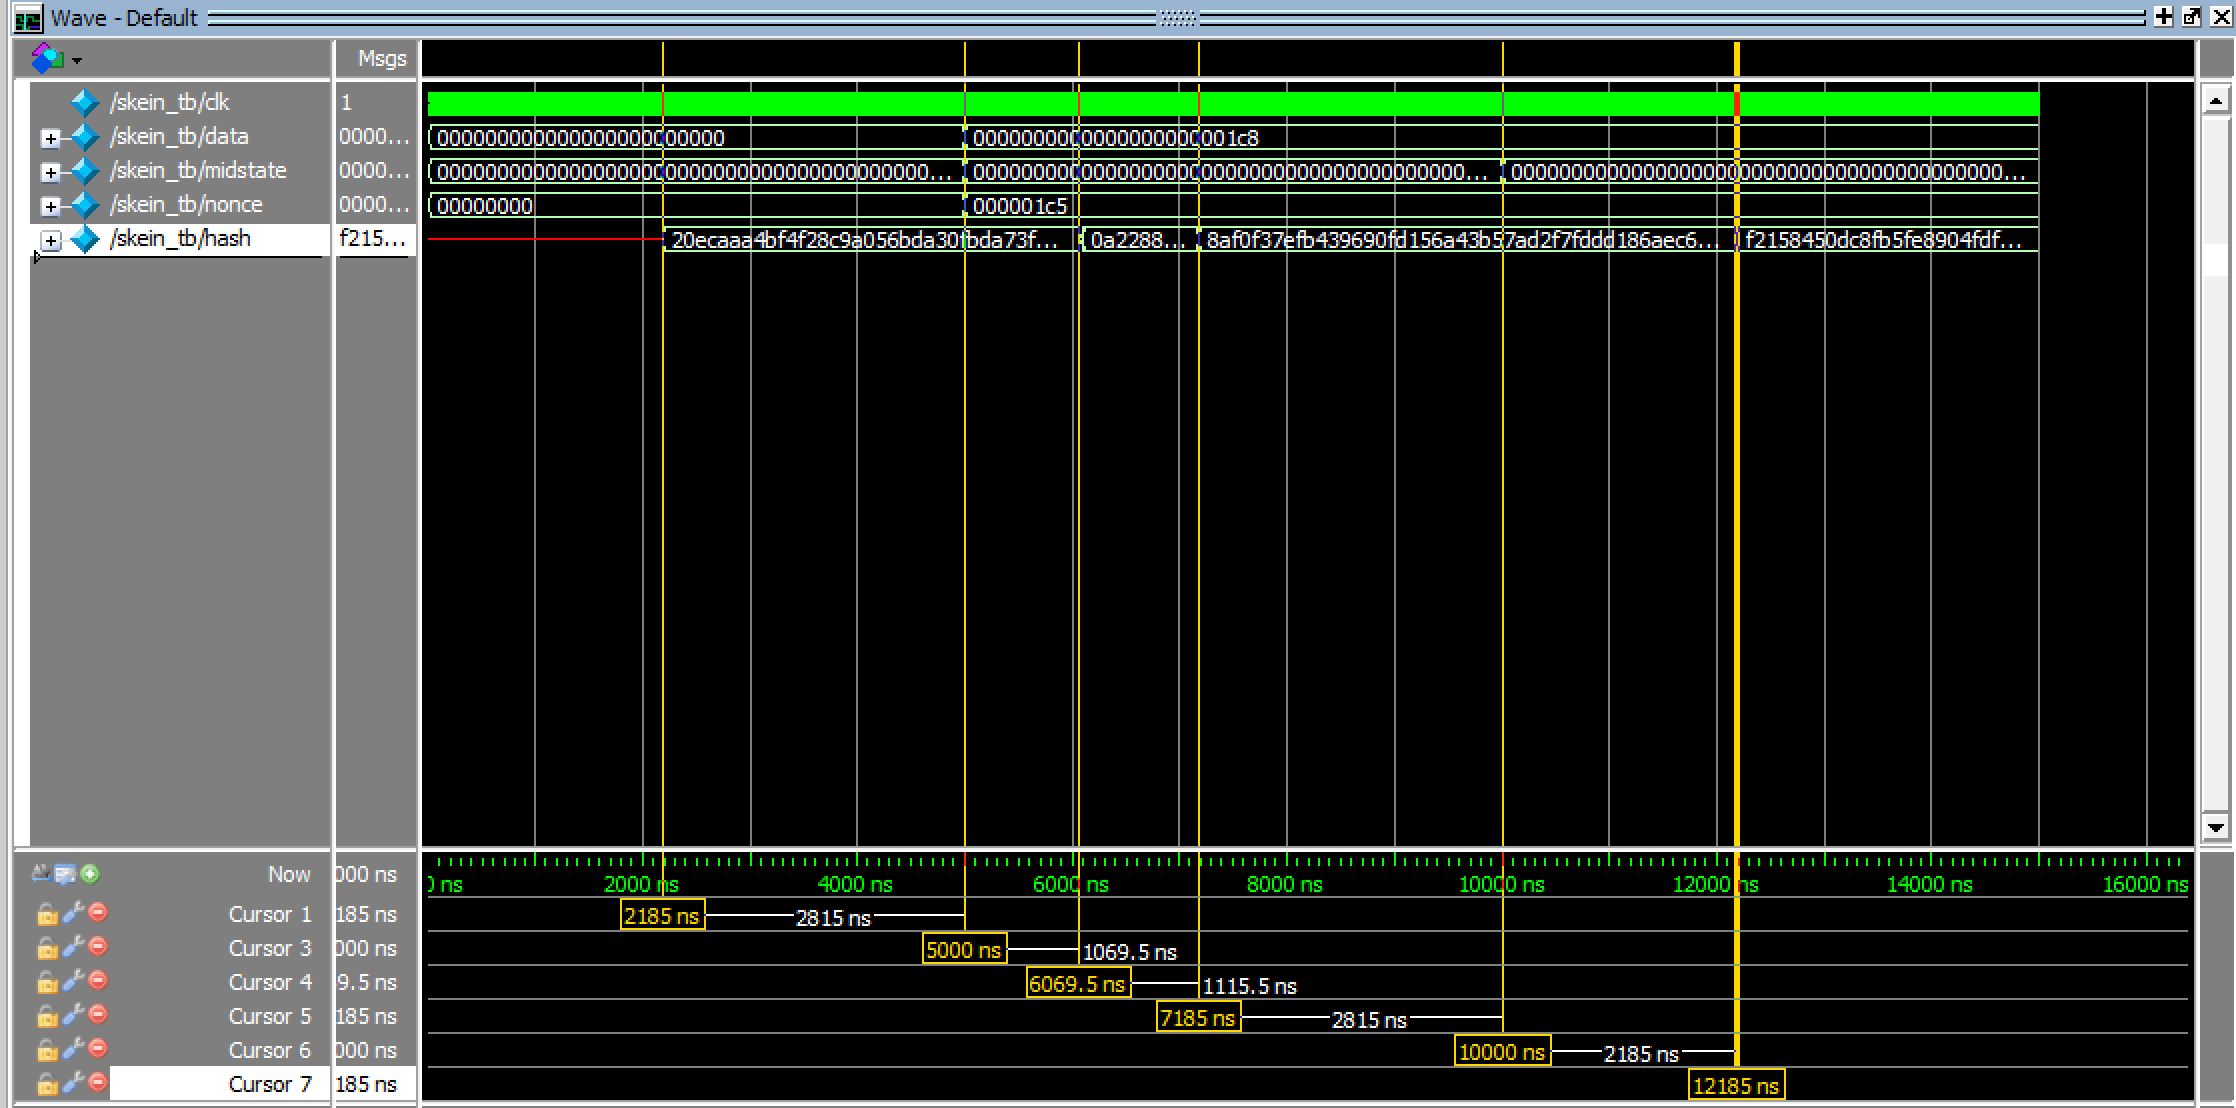
\includegraphics[width=16cm]{../RunData/sim_whole.png}	
	\caption{
	شکل موج مربوط به کل زمان شبیه‌سازی همراه با زمان‌های مهم
	}
\end{figure}
همان‌طور که مشخص است، هر‌بار که ورودی قطعه تغیر می‌کند، تقریبا ۲۸۱۵ نانو ثانیه طول می‌کشد که خروجی قطعه به حالت پایدار و نهایی خود برسد و قبل از این زمان خروجی قطعه ممکن است چندباری تغیر کند و مقدار درهم‌سازی نهایی نباشد، بنابر‌این در عمل این قطعه پس از
\textbf{ ۲۱۸ پالس ساعت }
جواب تولید خواهد کرد و درواقع ۲۱۸ پالس ساعت تاخیر دارد.

علت این مقدار تاخیر کاملا واضح است، طراحی انجام شده شامل ۷۲ 
\lr{round}
بوده و هر یک از این 
\lr{round}
ها دقیقا پس از ۴ کلاک خروجی خود را به بلاک بعدی انتقال می‌دهند. بنابر‌این
 $72 \times 4 = 218$ 
 کلاک طول خواهد کشید که جواب نهایی قطعه تولید شود، که این همان مقدار تاخیر مشاهده‌شده در شبیه‌سازی است.

\begin{figure}[H]
	\centering
	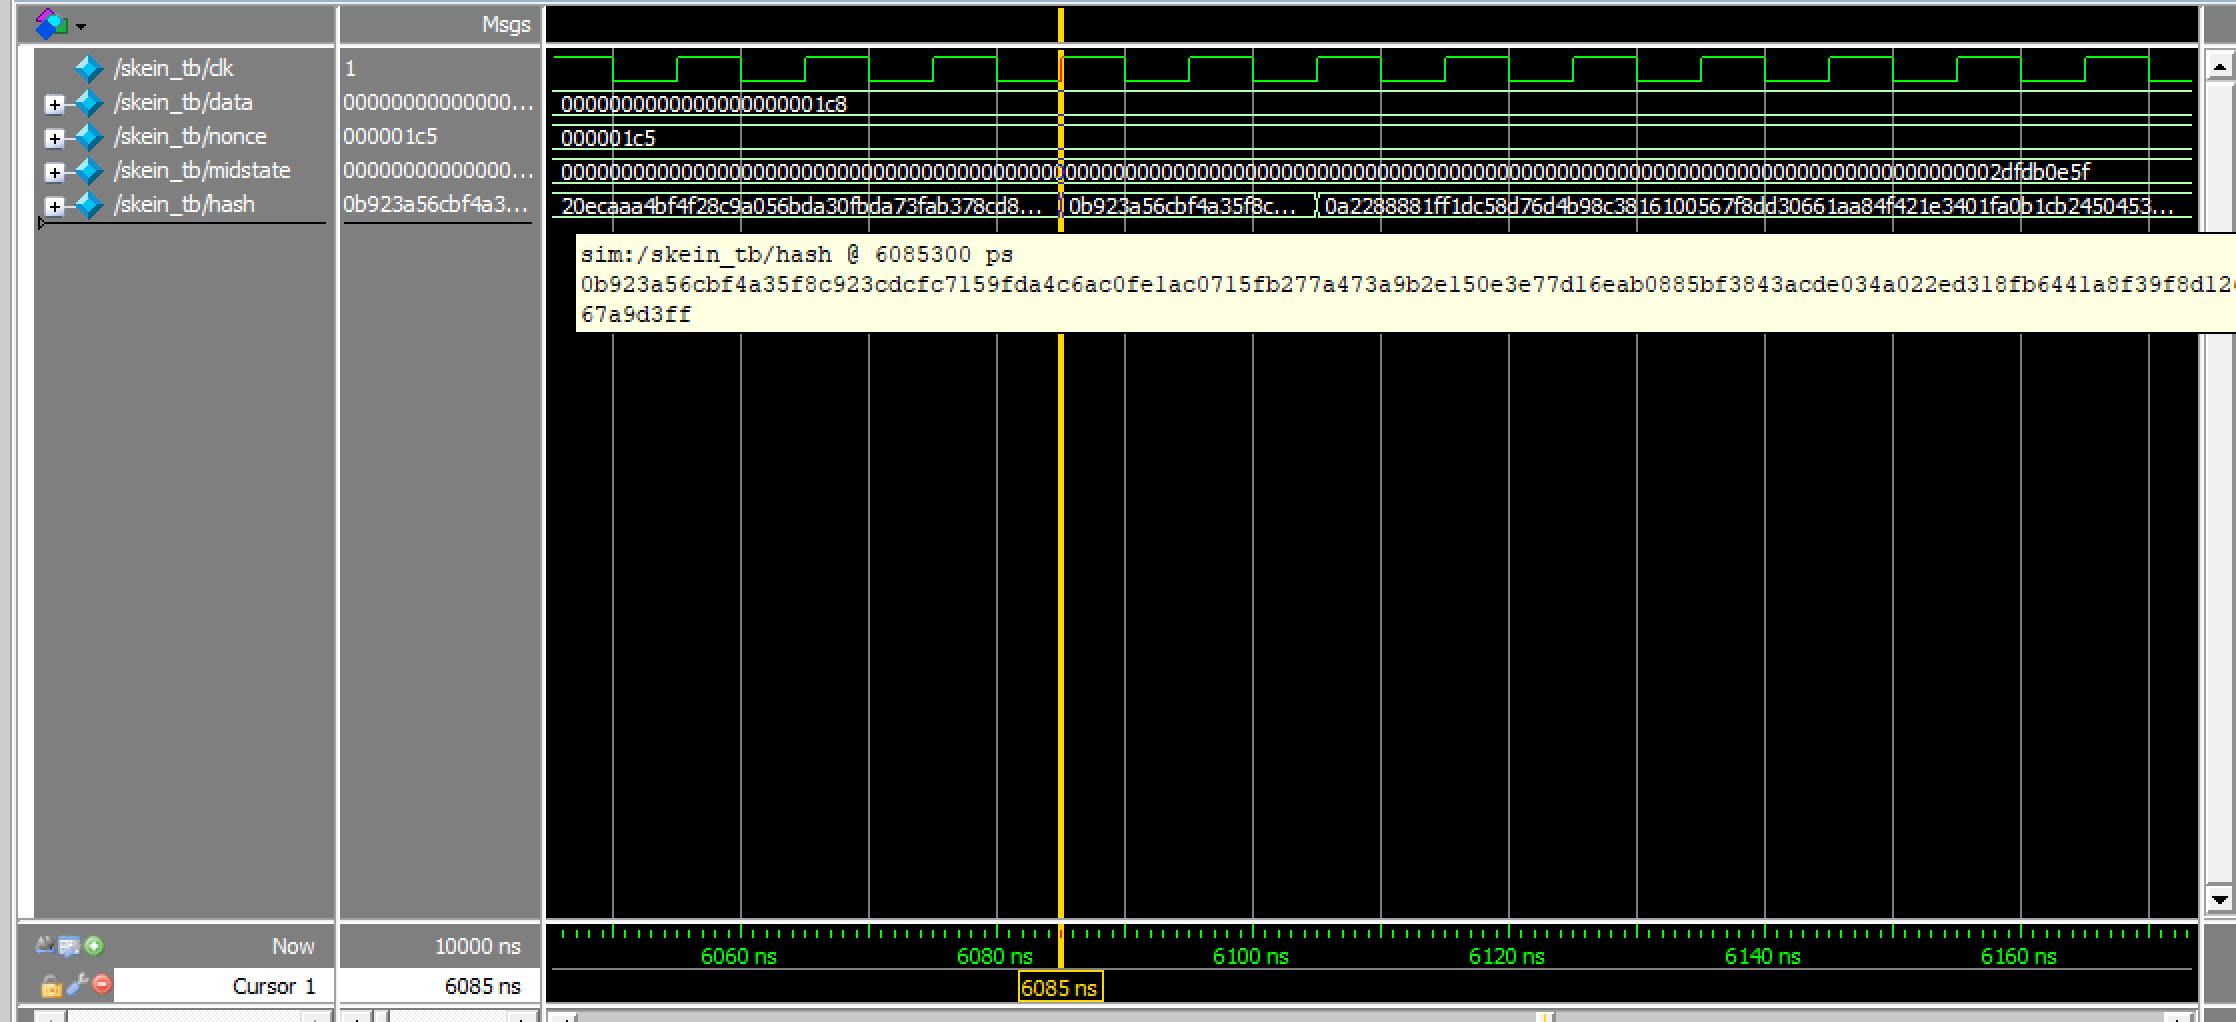
\includegraphics[width=16cm]{../RunData/sim_glitch1.png}	
	\caption{
		تولید خروجی غلط پیش از گذشت زمان ۲۱۸ پالس ساعت از لحظه‌ی تغیر ورودی
	}
\end{figure}
\begin{figure}[H]
	\centering
	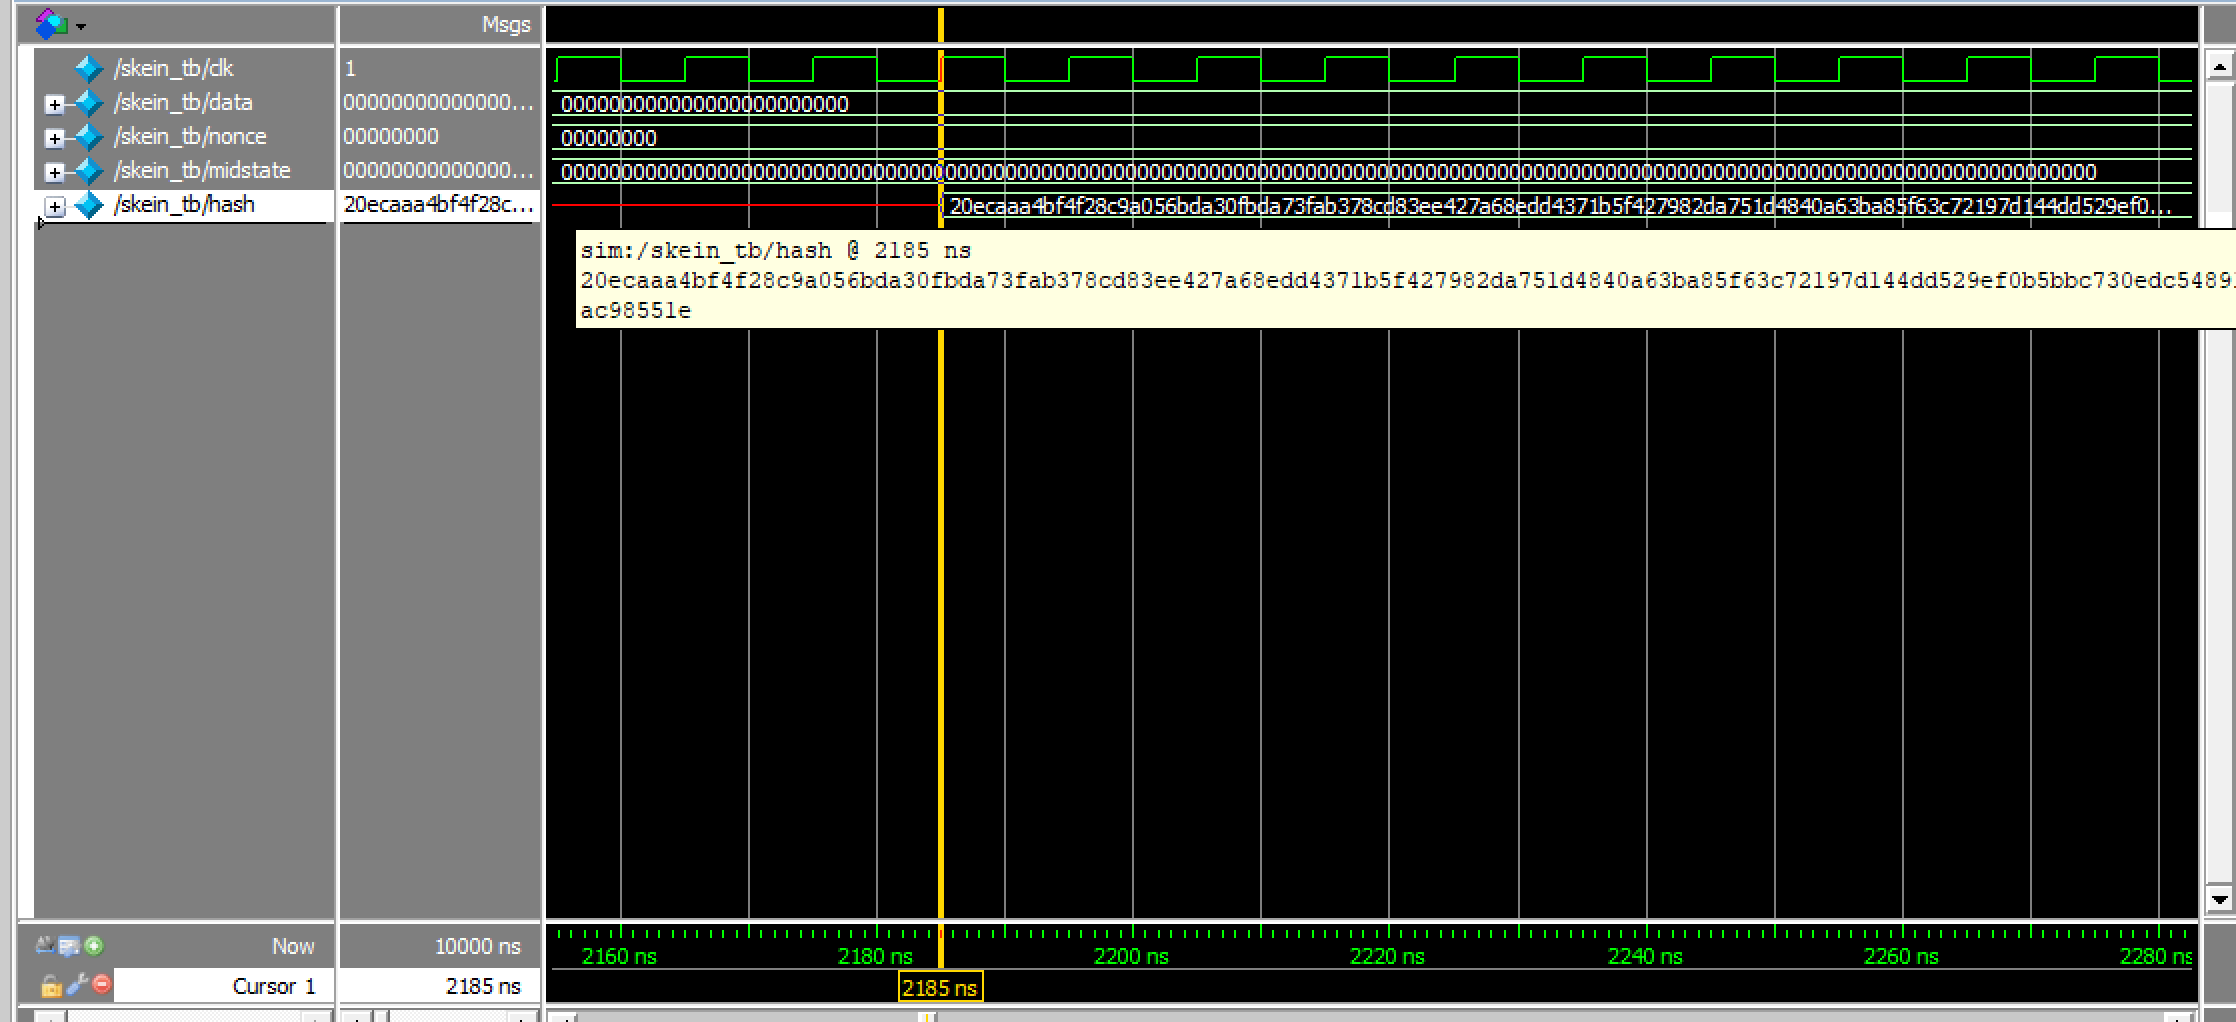
\includegraphics[width=16cm]{../RunData/sim_part1.png}	
	\caption{
		پاسخ تولید شده برای ورودی‌های صفر، پس از گذشت ۲۱۸ پالس ساعت
	}
\end{figure}
\begin{figure}[H]
	\centering
	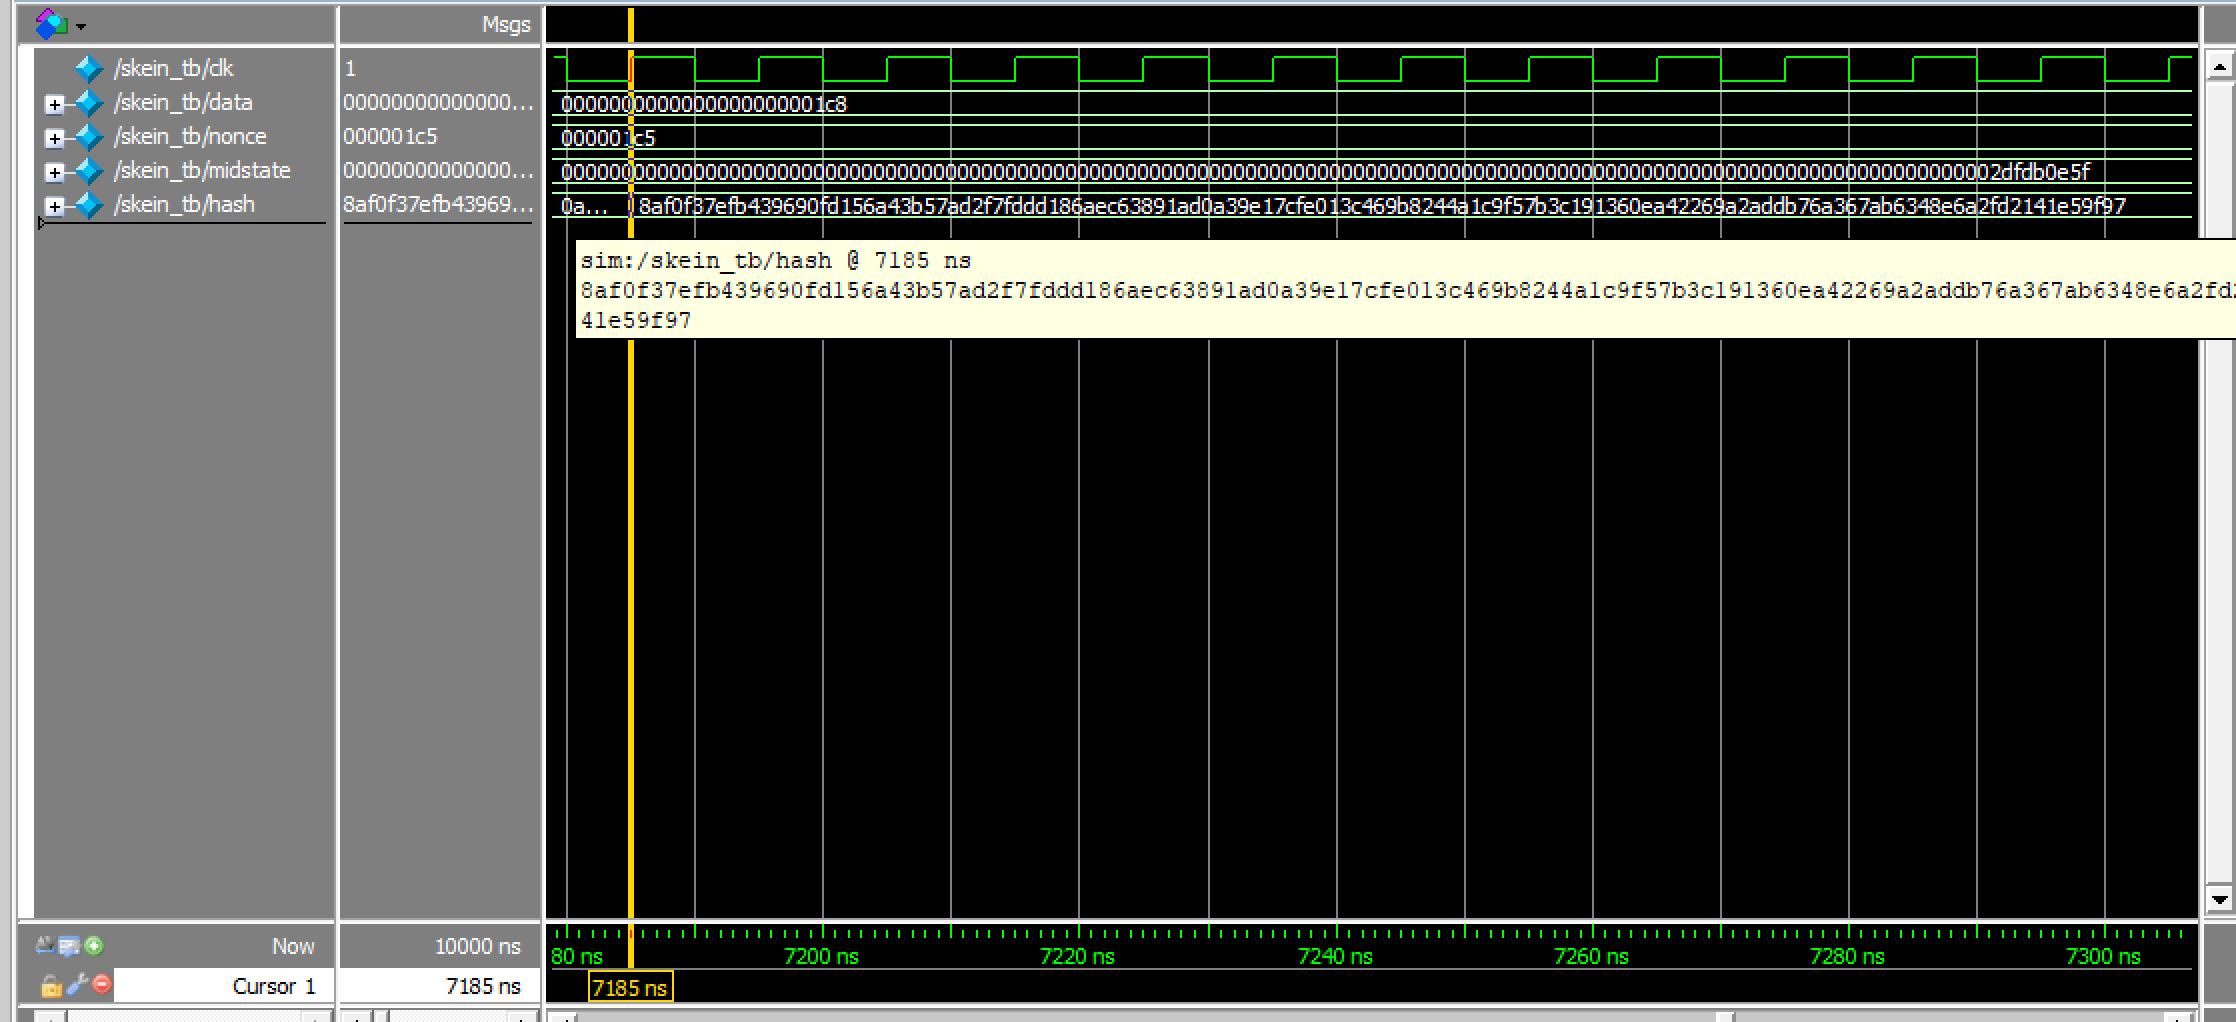
\includegraphics[width=16cm]{../RunData/sim_part2.png}	
	\caption{
		پاسخ تولید شده برای ورودی‌های داده شده پس از ۵۰۰۰ نانو ثانیه، پس از گذشت ۲۱۸ پالس ساعت
	}
\end{figure}
\begin{figure}[H]
	\centering
	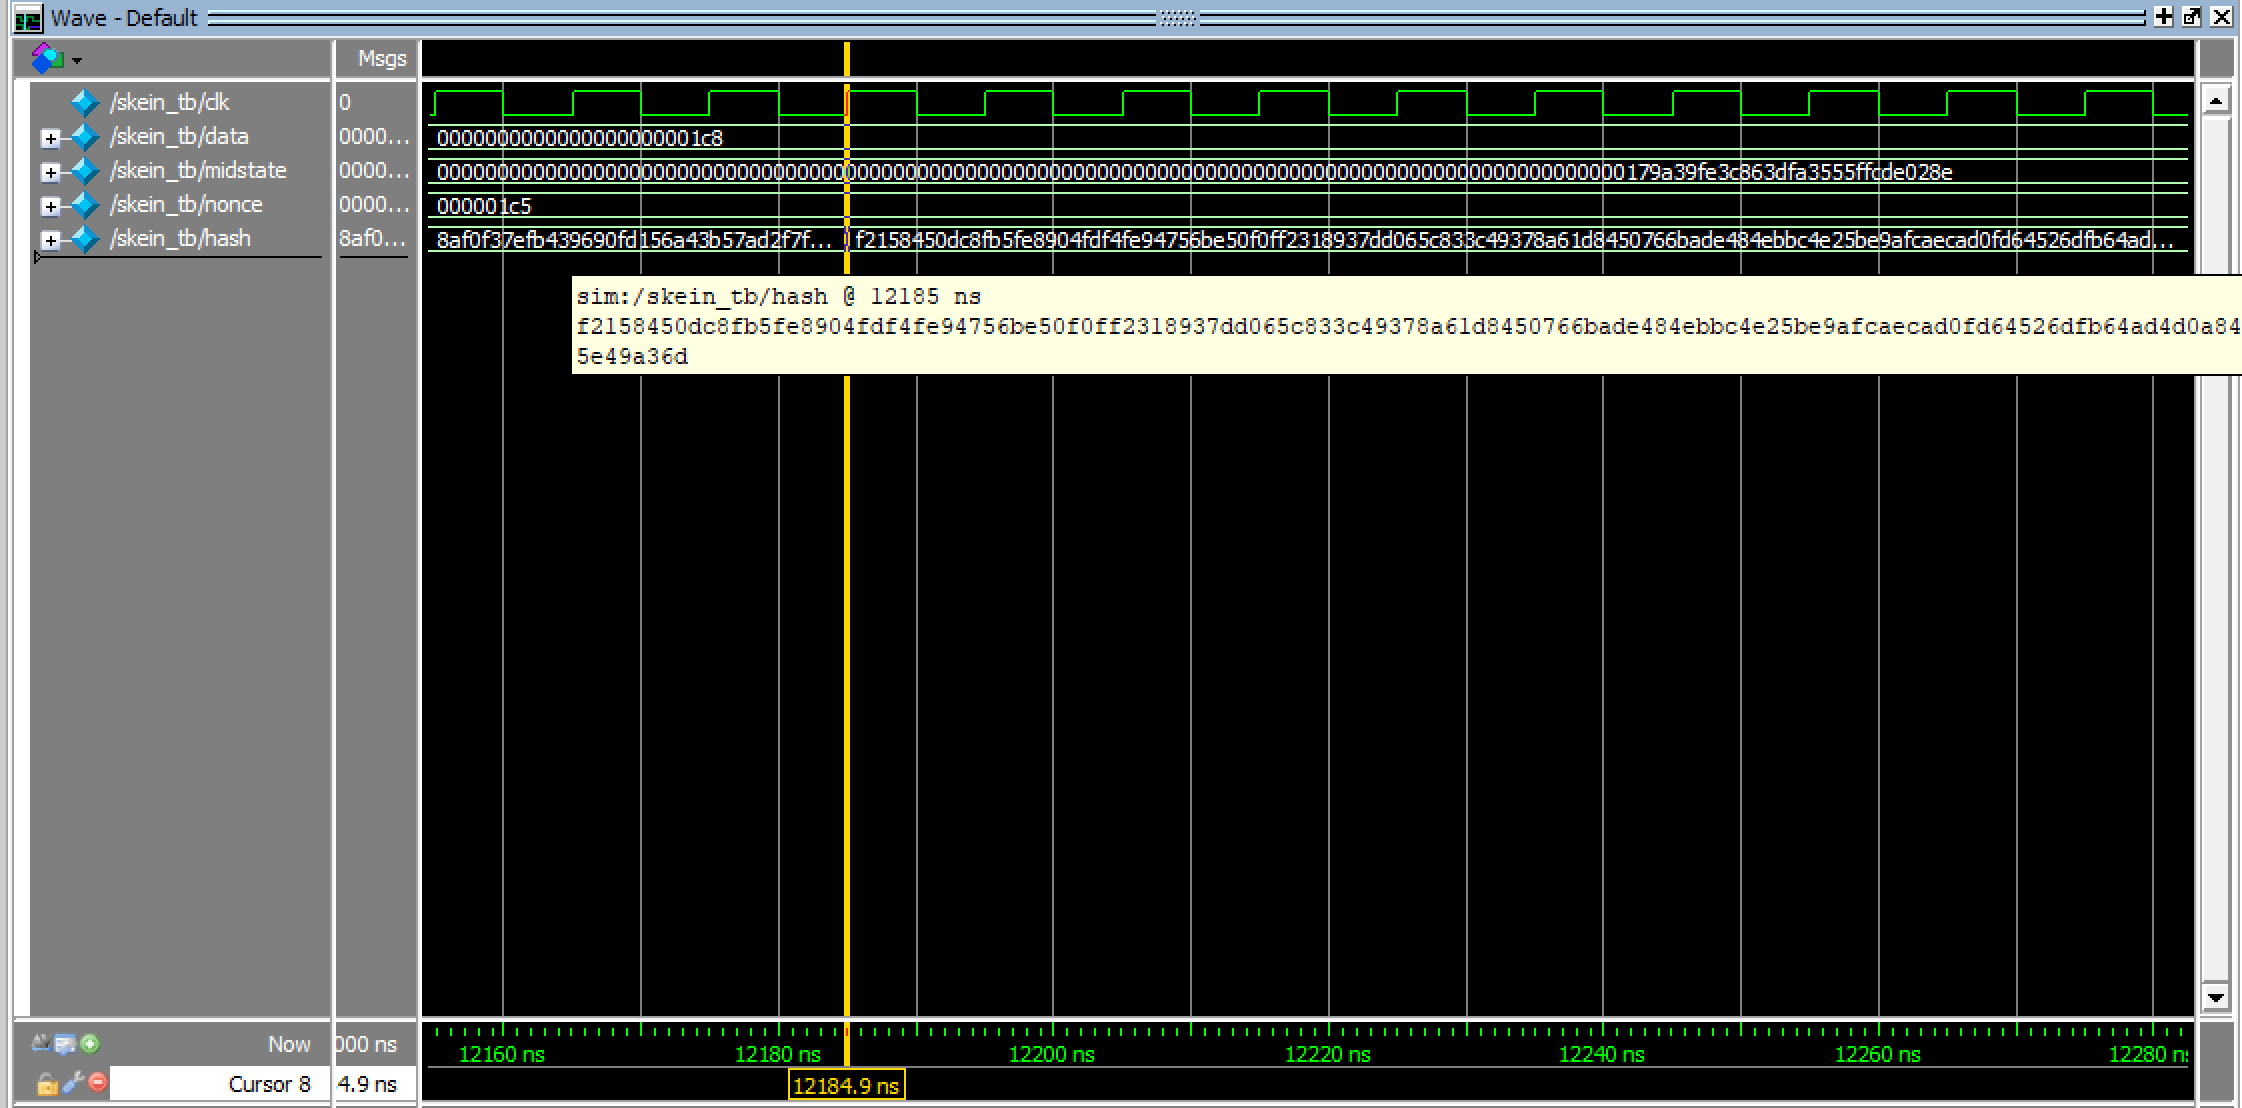
\includegraphics[width=16cm]{../RunData/sim_part3.png}	
	\caption{
		پاسخ تولید شده برای ورودی‌های داده شده پس از ۱۰۰۰۰ نانو ثانیه، پس از گذشت ۲۱۸ پالس ساعت
	}
\end{figure}

\pagebreak

\section{سنتز}
عمل سنتز به فرایند تبدیل طراحی سخت‌افزاری انجام شده با زبان‌های توصیف سخت‌افزار به لیستی از گیت‌های منطقی و ماژول هایی واقعی‌ای از رم‌ و رام ها و غیره برای تولید مدارات و قطعات \lr{ASIC}  و یا قرارگیری روی سخت‌افزار‌های از پیش‌آماده و قابل برنامه‌ریزی چون \lr{FPGA}‌ها گفته‌می‌شود. این‌کار توسط ابزاری نرم‌افزاری به نام 
\lr{Synthesis tool}
انجام پذیر‌است.

برای سنتز این پروژه برای محیط مقصد
\lr{xilinx}
، از
\lr{ ISE Design suite}
استفاده شد. درپیاده‌سازی تصحیح شده از الگوریتم، ماژول اصلی دارای 1153 
\lr{port}
 ورودی و خروجی می‌باشد، با توجه به این‌که هر قطعه‌ی \lr{FPGA} ای توان پشتیبانی از این تعداد
 \lr{I/O port}
 را ندارد،برای سنتز، پس از بررسی چند قطعه و با توجه به محدودیت های 
 \lr{licensing}
برخی از 
\lr{FPGA}
هایی که توان پیاده‌سازی این طراحی را داشتند، نهایتا از قطعه‌ی \lr{XC6VLX760} از خانواده‌ی \lr{Virtex6}
برای سنتز استفاده شد.

مراحل سنتز این پیاده‌سازی دچار هیچ پیغام خطایی نشد که لزومی به ارائه‌ی راه‌کار برای رفع آن باشد و تمامی فایل های خروجی غیر حجیم این سنتز از
\href{https://github.com/VahidZee/SkeinHashingHDL/blob/master/SynthesisFiles/}{
	 این آدرس
} 
قابل دسترسی می‌باشند.


\href{https://github.com/VahidZee/SkeinHashingHDL/blob/master/SynthesisFiles/report_summery.html}{
	این فایل
} 
شامل گزارشی کلی درباره ی این سنتز، اعم از درصد استفاده از سخت‌افزار‌های مختلف موجود در 
\lr{FPGA}
و غیره می باشد.

\href{https://github.com/VahidZee/SkeinHashingHDL/blob/master/SynthesisFiles/report_pinout.html}{
	این فایل
} 
شامل گزارشی از پورت‌های استفاده شده در 
\lr{FPGA}
برای اتصال ورودی و خروجی های قطعه‌ی طراحی شده است.

\href{https://github.com/VahidZee/SkeinHashingHDL/blob/master/SynthesisFiles/envsettings.html}{
	این فایل
} 
شامل گزارشی از تنظیمات محیط انجام سنتز در ابزار سنتز است.

\href{https://github.com/VahidZee/SkeinHashingHDL/blob/master/SynthesisFiles/report_pad.txt}{
	این فایل
} 
شامل گزارشی از مراحل 
\lr{placement}
و
\lr{format}
می باشد.


